\subsection{Differentiation of Measures}

\begin{definition} \label{def:lebesgue-averages-and-absolute-continuity} \hlt{Averages and Absolute Continuity}
\begin{enumerate}[label=(\roman*)]
\setlength{\itemsep}{0pt}
\item \hlt{Average}: for $f\in\mathscr{L}^1(E)$ and $A\subseteq E$, $m(A)>0$, set $[f:A]\defeq m(A)^{-1}\int_Af\,dm$.
\item \hlt{Density ratio}: for measurable $B$ and cube or ball $Q$, $m(Q)>0$, set $[B:Q]\defeq m(B\cap Q)/m(Q)$.
\item \hlt{Indefinite integral}: for $f\in\mathscr{L}^1([a,b])$, $F(x)=F(a)+\int_a^xf(t)\,dt$.
\item \hlt{Absolute continuity}: $F:[a,b]\to\R$ is absolutely continuous if $\forall\varepsilon>0,\exists\delta>0$,\\
finite disjoint $(a_j,b_j)\subseteq[a,b]$ satisfy $\sum_j(b_j-a_j)<\delta\Rightarrow\sum_j\abs{F(b_j)-F(a_j)}<\varepsilon$.
\end{enumerate}
\end{definition}

\begin{figure}[H]
  \centering
  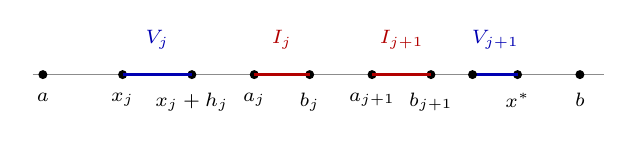
\begin{tikzpicture}[
  scale=0.88,
  every node/.style={font=\scriptsize},
  base/.style={black!45, line width=0.55pt},
  point/.style={circle, fill=black, inner sep=1.15pt},
  controlled/.style={blue!70!black, line width=1.25pt},
  gap/.style={red!70!black, line width=1.15pt},
  labelbox/.style={fill=white, inner sep=1pt}
]
  \draw[base] (-0.15,0) -- (8.1,0);

  \foreach \x/\lab in {
    0/a,
    1.15/x_j,
    2.15/{x_j+h_j},
    3.05/a_j,
    3.85/b_j,
    4.75/a_{j+1},
    5.60/b_{j+1},
    6.85/x^\ast,
    7.75/b
  } {
    \node[point] at (\x,0) {};
    \node[below=3pt] at (\x,0) {$\lab$};
  }

  \draw[controlled] (1.15,0) -- (2.15,0);
  \draw[gap] (3.05,0) -- (3.85,0);
  \draw[gap] (4.75,0) -- (5.60,0);
  \draw[controlled] (6.20,0) -- (6.85,0);
  \node[point] at (6.20,0) {};

  \node[labelbox, text=blue!70!black, above=8pt] at (1.65,0) {$V_j$};
  \node[labelbox, text=red!70!black, above=8pt] at (3.45,0) {$I_j$};
  \node[labelbox, text=red!70!black, above=8pt] at (5.18,0) {$I_{j+1}$};
  \node[labelbox, text=blue!70!black, above=8pt] at (6.53,0) {$V_{j+1}$};
\end{tikzpicture}

  \caption{Interval bookkeeping for absolute continuity.}
  \label{fig:absolute-continuity-interval-decomposition}
\end{figure}

\begin{perspective} \label{per:absolute-continuity-interval-bookkeeping} \hlt{Absolute Continuity as Interval Bookkeeping}\\
If $F(x)=\int_a^x f(t)\,dt$, by absolute continuity, disjoint intervals with small total length force small $F$ total change.\\
\end{perspective}

\begin{figure}[H]
  \centering
  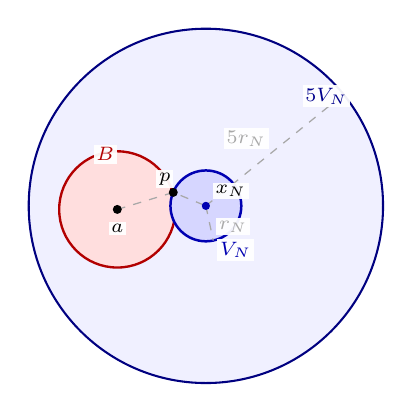
\begin{tikzpicture}[
  scale=0.90,
  every node/.style={font=\scriptsize},
  dilation/.style={draw=blue!50!black, fill=blue!6, line width=0.75pt},
  selected/.style={draw=blue!70!black, fill=blue!16, line width=0.9pt},
  missed/.style={draw=red!70!black, fill=red!13, line width=0.85pt},
  guide/.style={black!34, dashed, line width=0.45pt},
  point/.style={circle, fill=black, inner sep=1.15pt},
  center/.style={circle, fill=blue!70!black, inner sep=1.05pt},
  labelbox/.style={fill=white, fill opacity=0.94, text opacity=1, inner sep=1pt}
]
  \coordinate (x) at (0,0);
  \coordinate (a) at (-1.25,-0.05);
  \coordinate (p) at (-0.46,0.19);

  \draw[dilation] (x) circle (2.50);
  \draw[missed] (a) circle (0.82);
  \draw[selected] (x) circle (0.50);

  \draw[guide] (x) -- ++(39:2.50)
    node[pos=0.48, labelbox, above left=1pt] {$5r_N$};
  \draw[guide] (x) -- ++(-78:0.50)
    node[pos=0.60, labelbox, right=2pt] {$r_N$};
  \draw[guide] (a) -- (p) -- (x);

  \node[point] at (a) {};
  \node[center] at (x) {};
  \node[point] at (p) {};

  \node[labelbox, text=blue!70!black] at (0.42,-0.62) {$V_N$};
  \node[labelbox, text=blue!55!black] at (1.70,1.55) {$5V_N$};
  \node[labelbox, text=red!70!black] at (-1.42,0.73) {$B$};
  \node[labelbox] at (-0.58,0.38) {$p$};
  \node[labelbox] at (-1.25,-0.32) {$a$};
  \node[labelbox] at (0.35,0.21) {$x_N$};
\end{tikzpicture}

  \caption{A comparable missed ball lies inside the fivefold dilation of the selected ball.}
  \label{fig:vitali-fivefold-dilation}
\end{figure}

\begin{perspective} \label{per:vitali-covering-fivefold-control} \hlt{Vitali Covering Control}\\
Select balls disjointly by decreasing radius.\\
If $B$ is rejected, then $B\cap B_j\neq\emptyset$ for some earlier $B_j$ with $r(B)\leq r(B_j)$, hence $B\subseteq5B_j$.\\
\hlt{Key Insight}: Disjoint balls add; fixed dilations cover misses.
\end{perspective}

\begin{definition} \label{def:vitali-coverings-and-density-points} \hlt{Vitali Coverings and Density Points}
\begin{enumerate}[label=(\roman*)]
\setlength{\itemsep}{0pt}
\item For $A\subseteq M$, $\mathcal{V}$ is a \hlt{Vitali covering} of $A$ if $\forall p\in A,\forall r>0,\exists V\in\mathcal{V}$ with $p\in V$ and $\diam(V)<r$.
\item For measurable $E\subseteq\R^n$, its \hlt{density-point set} is $\operatorname{dp}(E)\defeq\{p\in\R^n:\lim_{Q\downarrow p}[E:Q]=1\}$, with $Q$ cubes, equivalently balls, shrinking to $p$.
\end{enumerate}
\end{definition}

\begin{theorem} \label{thm:vitali-covering-lemma-balls-cubes} \hlt{Vitali Covering Lemma for Balls and Cubes}\\
Let $E\subseteq\R^n$, $m^\ast(E)<+\infty$, and let $\mathcal{V}$ be a Vitali cover of $E$ by closed balls or axis-parallel cubes.\\
Then $\exists$ pairwise disjoint $(V_j)\subseteq\mathcal{V}$ with $m^\ast(E\setminus\bigcup_{j\geq1}V_j)=0$.
\begin{proof}
Fix open $O\supseteq E$ with $m(O)<m^\ast(E)+\varepsilon$, and replace $\mathcal{V}$ by $\{V\in\mathcal{V}:V\subseteq O\}$.\\
Greedily choose a maximal disjoint $(V_j)$ by dyadic diameter scales.\\
For a fixed dilation $V\mapsto V^\ast$, if $W\cap V\neq\emptyset$ and $\diam W\leq2\diam V$, then $W\subseteq V^\ast$ and $m(V^\ast)\leq C_nm(V)$.\\
Let $R=E\setminus\bigcup_jV_j$. Fix $N$ and $p\in R$.\\
Since $V_1,\ldots,V_N$ are closed, choose $W\in\mathcal{V}$ with $p\in W$ and $W\cap\bigcup_{j\leq N}V_j=\emptyset$. Maximality gives some $j>N$ with $W\cap V_j\neq\emptyset$ and comparable diameter, hence $p\in W\subseteq V_j^\ast$. Thus $R\subseteq\bigcup_{j>N}V_j^\ast$.\\
Therefore $m^\ast(R)\leq C_n\sum_{j>N}m(V_j)\to0$, because $\sum_jm(V_j)=m(\bigsqcup_jV_j)\leq m(O)<+\infty$. Hence $m^\ast(R)=0$.\\
\hlt{Structural Commentary}: Vitali selection gives a disjoint cover modulo null sets.\\
\hlt{Key Insight}: $R\subseteq\bigcup_{j>N}V_j^\ast$ and disjoint tails vanish.
\end{proof}
\end{theorem}

\begin{theorem} \label{thm:lebesgue-density-theorem} \hlt{Lebesgue Density Theorem}\\
For measurable $E\subseteq\R^n$, $\lim_{Q\downarrow p}[E:Q]=\mathbf{1}_E(p)$ for a.e. $p$, where $Q$ ranges over cubes, equivalently balls.\\
Equivalently, $m(E\triangle\operatorname{dp}(E))=0$.
\begin{proof}
Assume $m(E)<+\infty$. For $a\in(0,1)$ set $E_a\defeq\{p\in E:\liminf_{Q\downarrow p}[E:Q]<a\}$.\\
Cubes $Q\ni p$ with $[E:Q]<a$ form a Vitali cover of $E_a$. For open $O\supseteq E_a$ with $m(O)<m(E_a)+\varepsilon$, Theorem \ref{thm:vitali-covering-lemma-balls-cubes} gives disjoint $(Q_j)\subseteq O$ covering $E_a$ modulo null sets.\\
Hence $m(E_a)\leq\sum_jm(E_a\cap Q_j)\leq\sum_jm(E\cap Q_j)<a\sum_jm(Q_j)\leq a\,m(O)<a(m(E_a)+\varepsilon)$.\\
Let $\varepsilon\downarrow0$; since $a<1$, $m(E_a)=0$. Thus $p\in E\setminus\bigcup_{a\in\Q\cap(0,1)}E_a$ has density $1$. Apply same argument to bounded pieces of $E^c$ to get density $0$ a.e. on $E^c$; then exhaust arbitrary $E$ by bounded pieces.\\
\hlt{Structural Commentary}: Measurable sets are locally $0$ or $1$ a.e.\\
\hlt{Key Insight}: Vitali turns bad density into $m(E_a)\le a\,m(E_a)$.
\end{proof}
\end{theorem}

\begin{corollary} \label{cor:density-points-commute-with-slices} \hlt{Density Points Commute with Slicing Almost Everywhere}\\
Let $E\subseteq\R^n\times\R^k$ be measurable. For a.e. $x\in\R^n$, $\operatorname{dp}(E_x)=\{y:(x,y)\in\operatorname{dp}(E)\}$ up to a null subset of $\R^k$.
\begin{proof}
Set $D=\operatorname{dp}(E)$ and $N=E\triangle D$.\\
By Theorem \ref{thm:lebesgue-density-theorem}, $m_{n+k}(N)=0$; hence Theorem \ref{thm:zero-slices-null-set-criterion} gives $m_k(N_x)=0$ for a.e. $x$.\\
Intersecting with the Fubini good set, $E_x,D_x$ are measurable and $m_k(E_x\triangle D_x)=m_k((E\triangle D)_x)=0$.\\
Applying Theorem \ref{thm:lebesgue-density-theorem} in $\R^k$ gives $m_k(E_x\triangle\operatorname{dp}(E_x))=0$.\\
Therefore $m_k(\operatorname{dp}(E_x)\triangle D_x)=0$; and $m_k(\operatorname{dp}(E_x)\triangle D_x)=0$.
This is the claimed equality modulo null sets.\\
\hlt{Structural Commentary}: Almost-everywhere local fullness is compatible with almost-everywhere slicing.\\
\hlt{Key Insight}: Null ambient errors have null slices for almost every base point.
\end{proof}
\end{corollary}

\begin{lemma} \label{lem:large-average-set-bound} \hlt{Large Averages Have Small Outer Measure}\\
For a cube $Q_0\subseteq\R^n$, $g\ge0$ in $\mathscr{L}^1(Q_0)$, and $\lambda>0$,\\
set $A_\lambda\defeq \left\{p\in Q_0:\forall r>0\ \exists\text{ cube }Q\subseteq Q_0,\ p\in Q,\ \diam Q<r,\ [g:Q]>\lambda\right\}$ for $m^\ast(A_\lambda)\leq \frac{1}{\lambda}\int_{Q_0} g$.
\begin{proof}
Let $\mathcal{V}_\lambda=\{Q\subseteq Q_0:Q\text{ is a cube and }[g:Q]>\lambda\}$. By definition, $\mathcal{V}_\lambda$ is a Vitali cover of $A_\lambda$; choose disjoint $(Q_j)\subseteq\mathcal{V}_\lambda$ with $m^\ast(A_\lambda\setminus\bigcup_jQ_j)=0$. Then $\lambda m^\ast(A_\lambda) \le \lambda\sum_jm(Q_j) <\sum_j\int_{Q_j}g \le\int_{Q_0}g$.\\
\hlt{Structural Commentary}: Weak type for local averages.\\
\hlt{Key Insight}: Disjoint Vitali cubes turn pointwise large averages into one integral bound.
\end{proof}
\end{lemma}

\begin{theorem} \label{thm:lebesgue-average-value-theorem} \hlt{Lebesgue Average Value Theorem}\\
For $f\in\mathscr{L}^1_{\mathrm{loc}}(\R^n)$, $\lim\limits_{Q\downarrow p}[f:Q]=f(p)$ for a.e. $p\in\R^n$ with $Q$ cubes, equivalently balls, shrinking to $p$.
\begin{proof}
Fix a cube $Q_0$; it suffices to prove the claim for a.e. $p\in Q_0^\circ$.\\
For $\alpha>0$, let $B_\alpha=\left\{p\in Q_0^\circ:\limsup\limits_{Q\downarrow p}|[f:Q]-f(p)|>\alpha\right\}$.\\
Choose $h\in C(Q_0)$ with $\|f-h\|_{L^1(Q_0)}<\eta$, and set $g=|f-h|$. Since $[h:Q]\to h(p)$, $B_\alpha\subseteq \{g>\alpha/3\}\cup A_{\alpha/3}(g)$.\\
By Markov and Lemma \ref{lem:large-average-set-bound}, $m^\ast(B_\alpha)\le \frac{3}{\alpha}\int_{Q_0}g+\frac{3}{\alpha}\int_{Q_0}g <\frac{6\eta}{\alpha}$.\\
Let $\eta\downarrow0$; then $m(B_\alpha)=0$. Count over $\alpha\in\Q_{>0}$ and exhaust $\R^n$ by cube interiors.\\
\hlt{Structural Commentary}: Local averages recover the original integrable function almost everywhere.\\
\hlt{Key Insight}: Continuous approximation handles the good part; Vitali's estimate makes the bad part small.
\end{proof}
\end{theorem}

\begin{theorem} \label{thm:lebesgue-antiderivative-theorem} \hlt{Lebesgue's Antiderivative Theorem}\\
For $f\in\mathscr{L}^1([a,b])$, define $F(x)=c+\int_a^x f(t)\,dt$. Then $F\in AC([a,b])$ and $F'(x)=f(x)$ for a.e. $x\in[a,b]$.
\begin{proof}
Given $\varepsilon>0$, choose $\delta>0$ so that $m(A)<\delta$ implies $\int_A|f|<\varepsilon$.\\
If $(\alpha_j,\beta_j)$ are disjoint and $\sum_j(\beta_j-\alpha_j)<\delta$, then $\sum_j|F(\beta_j)-F(\alpha_j)| \le \sum_j\int_{\alpha_j}^{\beta_j}|f| =\int_{\bigcup_j(\alpha_j,\beta_j)}|f| <\varepsilon$, so $F\in AC([a,b])$. For $x,x+h\in[a,b]$, let $I_h(x)=(\min\{x,x+h\},\max\{x,x+h\})$.\\
Then $\frac{F(x+h)-F(x)}{h}=[f:I_h(x)]$. Extending $f$ by $0$ outside $[a,b]$, Theorem \ref{thm:lebesgue-average-value-theorem} in one dimension gives $[f:I_h(x)]\to f(x)$ for a.e. $x$. Hence $F'=f$ a.e.\\
\hlt{Structural Commentary}: The indefinite Lebesgue integral is the correct antiderivative for integrable functions.\\
\hlt{Key Insight}: Differentiating the integral is the same as shrinking the averaging interval.
\end{proof}
\end{theorem}
